\documentclass{beamer}

\usepackage{graphicx}
\usetheme{default}

\title{ShuttleQL}
\subtitle{SE464 Project Proposal}
\author{Clement Hoang \and David Dong \and Jason Fang \and Tony Lu}
\institute{University of Waterloo}
\date{Fall 2016}

\begin{document}

\begin{frame}
  \titlepage
\end{frame}

\section{Problem}

\begin{frame}{Problem}
  \begin{itemize}
  \item {
    our target are \alert{badminton clubs} throughout the world
  }
  \item {
    there is currently no unified solution to \alert{club management} and \alert{court management}
  }
  \item {
    it is very tough to \alert{improve} your play unless you hire a coach
  }
  \item {
    many tasks have to be done \alert{manually} which leads to \alert{player dissatisfaction} and \alert{operation inefficiency}
    \begin{itemize}
        \item
          Club members are manually recorded onto Excel spreadsheets
        \item
          Club executives have to manually time rotations and move players on and off courts accordingly
        \item
          During rotation, players crowd around the board to see which court they are on
    \end{itemize}
  }
  \end{itemize}
\end{frame}

\section{Solution}

\begin{frame}{Enter ShuttleQL}

  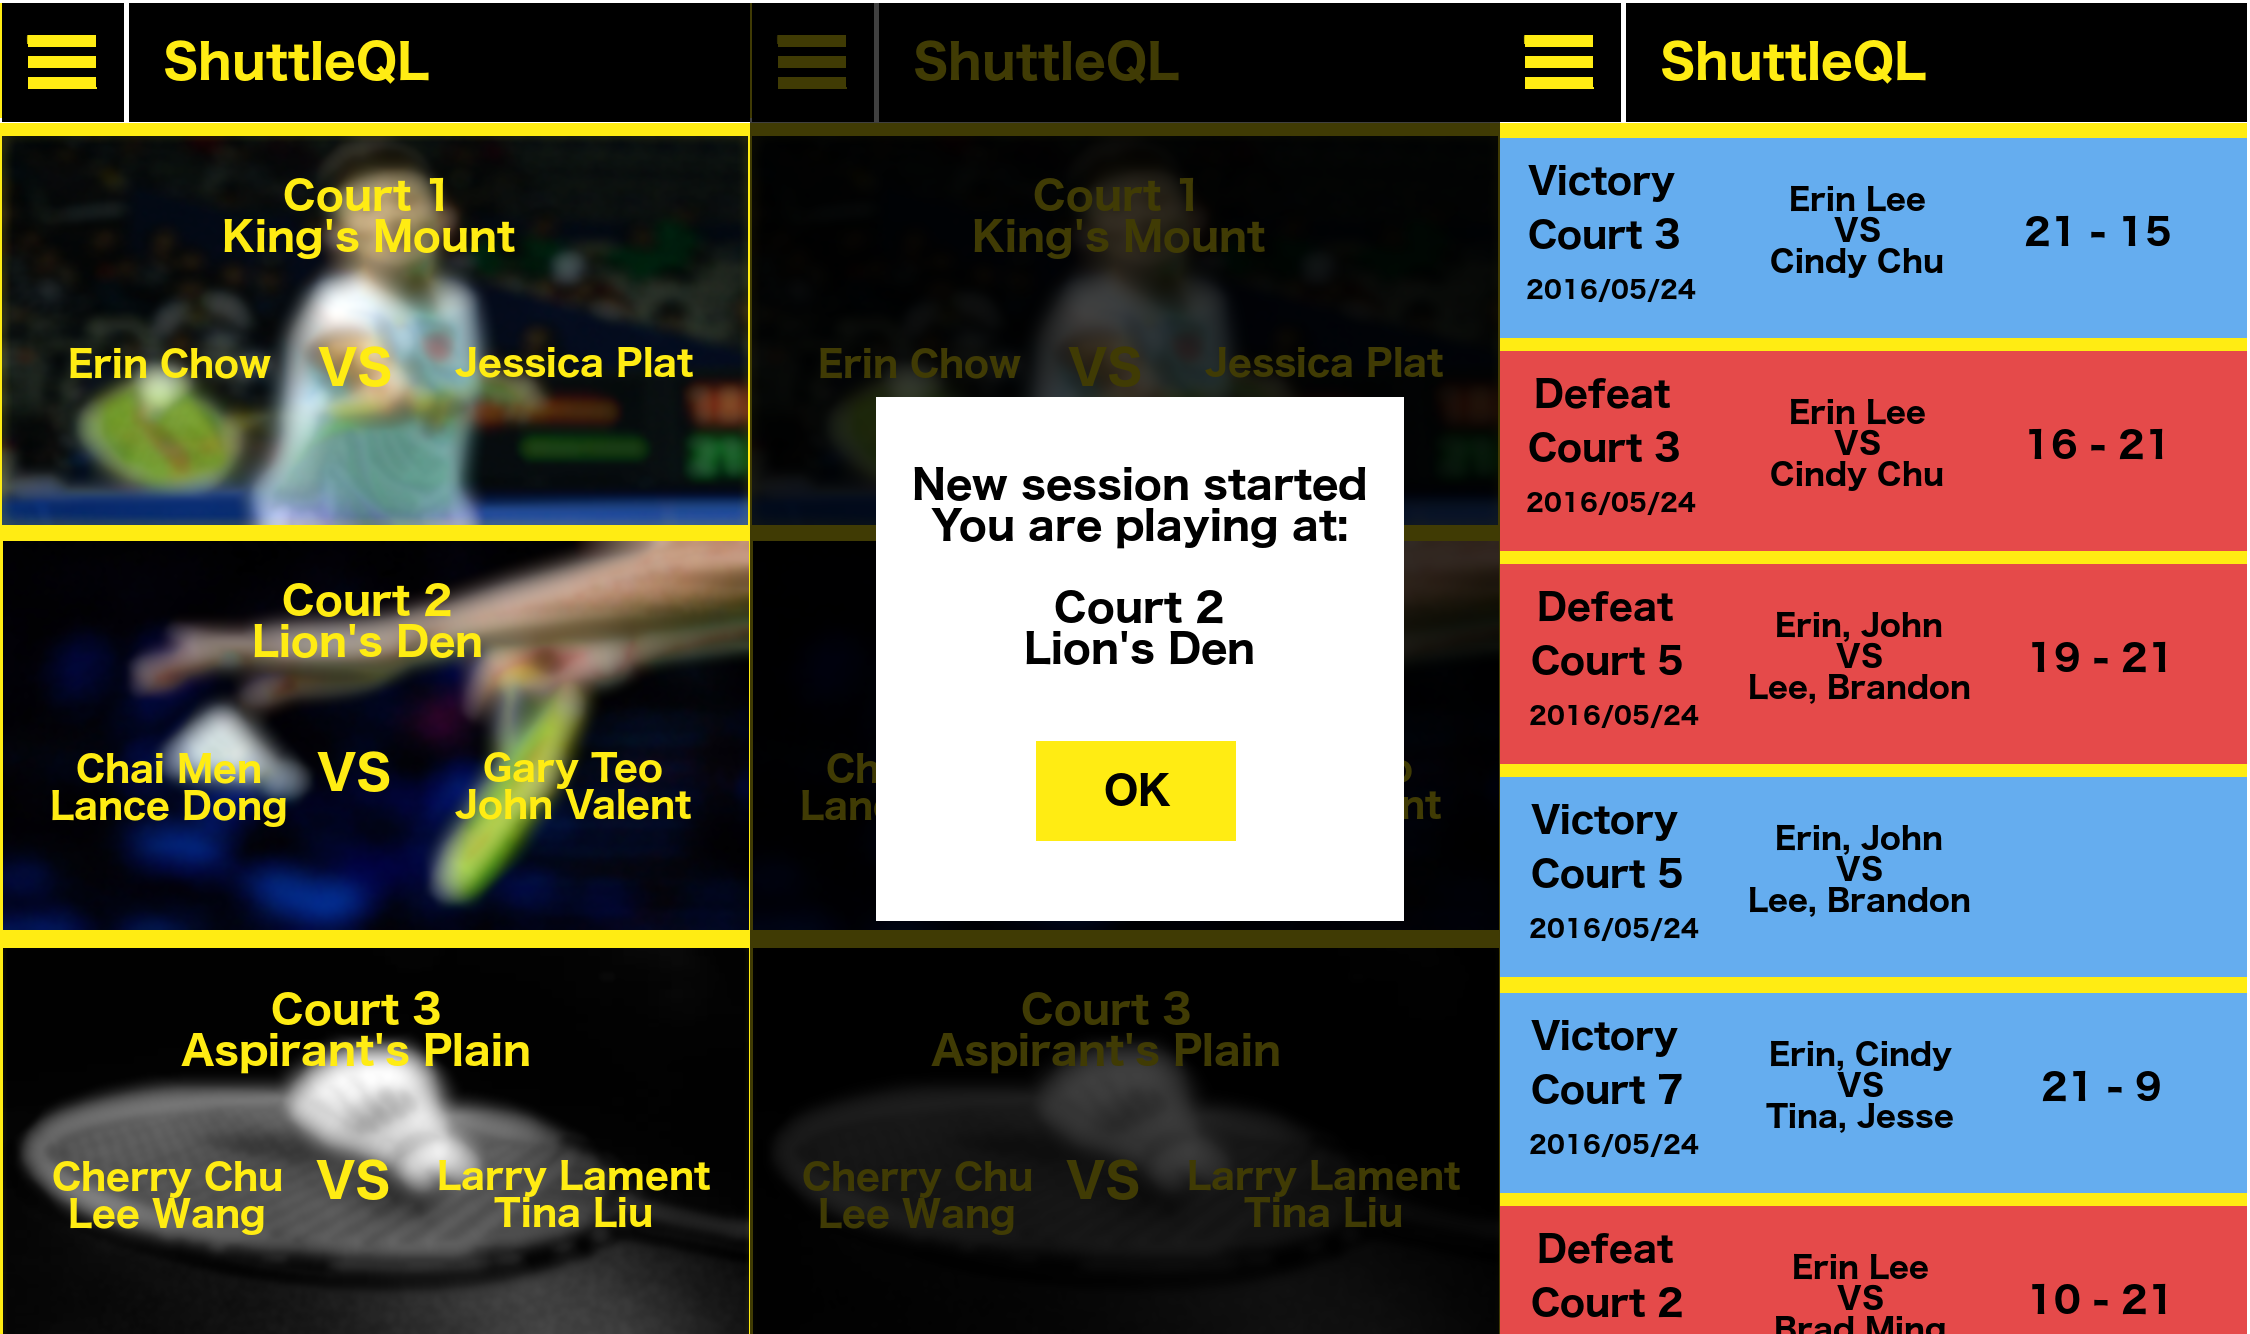
\includegraphics[width=11cm]{combined}

\end{frame}

\section{Features}

\begin{frame}{Features}
\begin{block}{Automated Management}
    \begin{itemize}
        \item Streamlined registration for new club members
        \item Matchmaking and court changes would be decided by the system
    \end{itemize}
\end{block}
\begin{block}{Centralized Hub}
    \begin{itemize}
        \item Announcements can be broadcast on the website
        \item Push notifications to users during court change and important notices
    \end{itemize}
\end{block}
\begin{block}{Player Improvement}
    \begin{itemize}
        \item Track player match history
        \item Bystander referee system for challenge games
        \item Visualizations to see performance over time
    \end{itemize}
\end{block}
\end{frame}

\section*{End}

\begin{frame}
    \begin{block}{}
    Thank you for your time!
    \end{block}
\end{frame}

\end{document}
